\section{Physik der Gitarre}

\subsection{Vorwort}


\subsection{Versuchsaufbau}

Die Gitarre liegt auf einer Polsterung auf dem Tisch. Das Mirkofon wird mit einem Stativ mittig oberhalb des Schallochs der Gitarre platziert. Das Mikrofon wird auf Amplitudenmodus gestellt und mit dem Sensor-CASSY wird die Ausgangsspannung des Mirkofons gemesssen. Vor der Messung wird die Gitarre mit einem Stimmgerät mit Stimmgenauigkeit von $\pm 1 \, \mathrm{Cent}$ gestimmt.


\subsection{Messung der Schwebung}


\subsubsection{Versuchsdurchführung}

Nach dem Stimmen der Gitarre wird die A-Saite leicht verstimmt. Anschließend wird die offene D-Saite zusammen mit der im 5. Bund gegriffenen A-Saite angeschlagen und eine Messung mit dem Mikrofon gestartet. Es werden für vier verschiedene Verstimmungen Messungen aufgenommen. Dabei wird für die erste Verstimmung eine Messung aufgenommen und für die restlichen drei jeweils zwei Messungen. Für die ersten beiden, sowie die letzte Messung hat das Sensor-CASSY folgende Messparameter:
\begin{enumerate}[-]
\item Messbereich: $-10$ bis $10\,$V
\item Intervall: $200\,\mu$s
\item Messungen: $16000$
\item Messzeit: $3.2\,$s
\end{enumerate}
Für die anderen Messungen werden folgende Messparameter verwendet:
\begin{enumerate}[-]
\item Messbereich: $-10$ bis $10\,$V
\item Intervall: $500\,\mu$s
\item Messungen: $16000$
\item Messzeit: $8\,$s
\end{enumerate}


\subsubsection{Versuchsauswertung}

Die Rohdaten der Messung sind exemplarisch in Abbildung \ref{rohSch} zu sehen.

\begin{figure}[h]
	\centering
	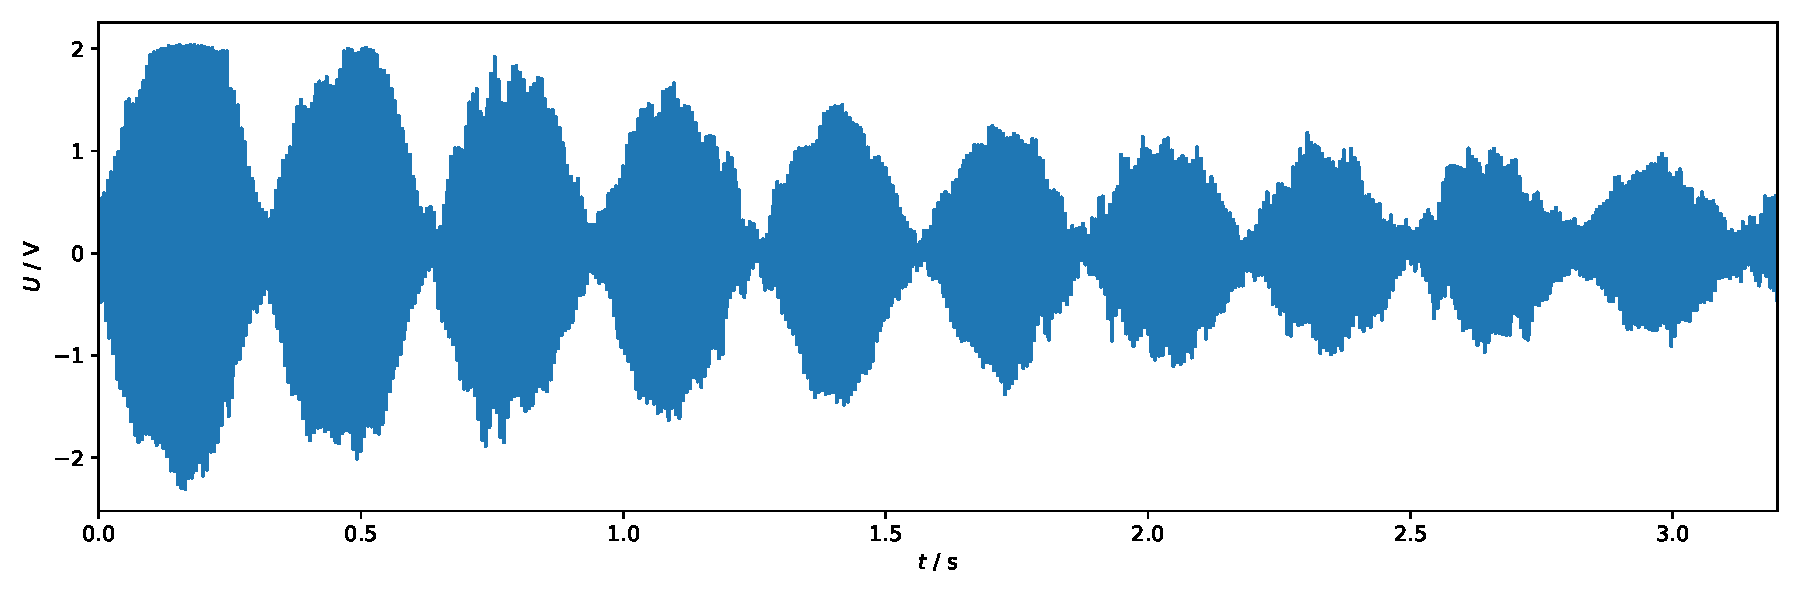
\includegraphics[width=\linewidth]{plots/rohdaten_schwebung.pdf}
	\caption{Visualisierung der Rohdaten aus der ersten Messung (\mbox{``schwebung\_1.lab''})}
	\label{rohSch}
\end{figure}

Wir bestimmen nun die Schwebungsfrequenz $f_S$ und die Frequenz der resultierenden Schwingung $f_R$ auf zwei unterschiedliche Arten. Zum einen durch Ablesen von Maxima/Minima aus den Rohdaten und zum anderen durch eine Fast Fourier Transformation (FFT) der Rohdaten. 
In der ersten Variante werden die Maxima/Minima per Augenmaß aus Plots der Rohdaten abgelesen, wie es in Abbildung \ref{MaxAblesen} zu sehen ist. Um eine Unabhängigkeit der daraus erhaltenen Werte zu erreichen wird aus den Dateien \mbox{``schwebung\_1.lab''}, \mbox{``schwebung\_2.1.lab''}, \mbox{``schwebung\_3.2.lab''} und \mbox{``schwebung\_4.2.lab''} abgelesen und die FFT auf die Daten aus den Dateien \mbox{``schwebung\_1.lab''}, \mbox{``schwebung\_2.2.lab''}, \\
\mbox{``schwebung\_3.1.lab''} und \mbox{``schwebung\_4.1.lab''} angewendet.

\begin{figure}[h]
	\centering
	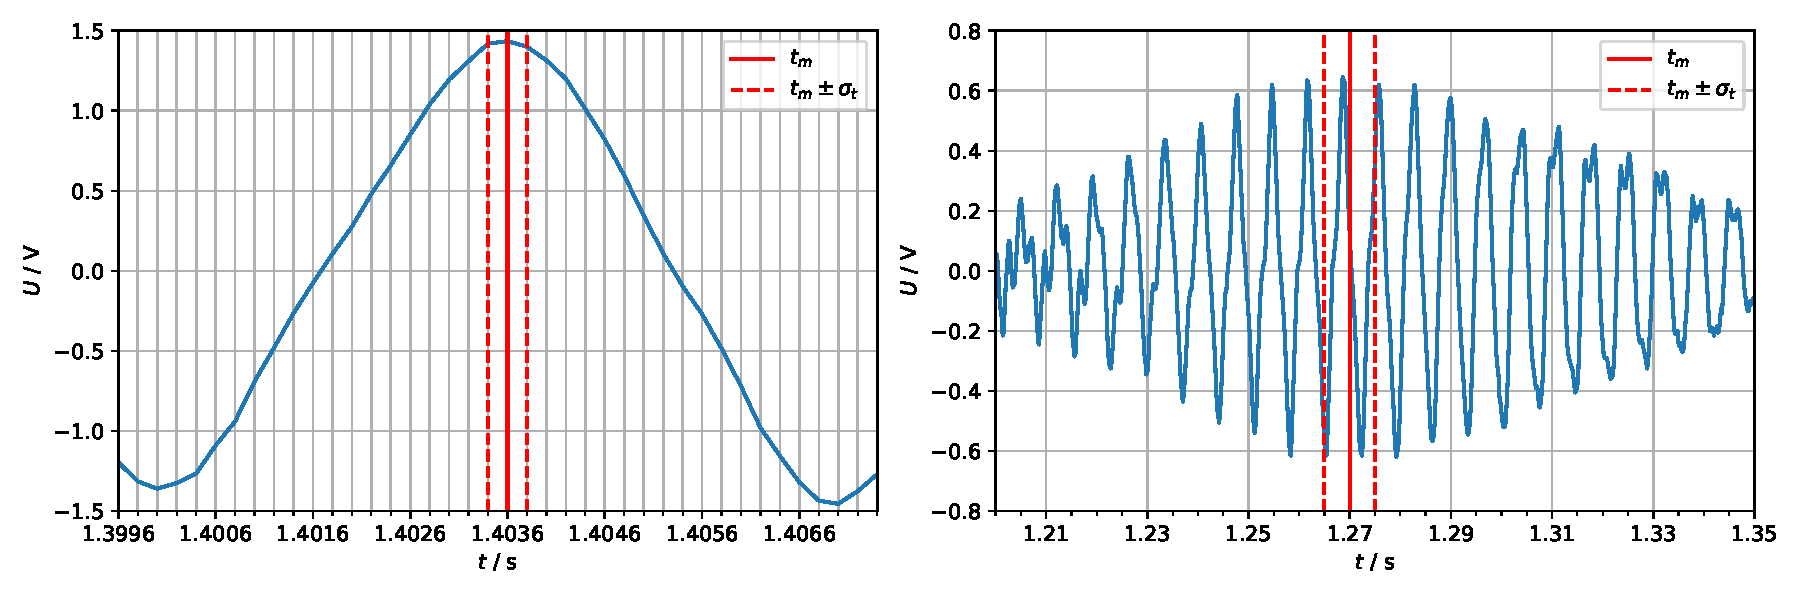
\includegraphics[width=\linewidth]{plots/bspMaxima.pdf}
	\caption{Bestimmung der Maxima aus den Rohdaten}
	\label{MaxAblesen}
\end{figure}
Beim Ablesen für die resultierende Schwingung ist zu beachten, dass sich bei einem Nulldurchgang der Schwebungschwingung die Art das Extremums, welches wir ablesen wollen, ändert. Die so abgelesenen Zeitpunkte sind in Tabelle \ref{tabTimeRes} dokumentiert. Angesichts der Messintervalle für die Zeit und der Erkennbarkeit der Extrema werden für die Schwebungen 1 und 2 die Zeitunsicherheit $\sigma_t = 0.2 \, \mathrm{ms}$, für die Schwebung 3 $\sigma_t = 0.5 \, \mathrm{ms}$ und für Schwebung 4 $\sigma_t = 0.4 \, \mathrm{ms}$ angesetzt.

\begin{table}[H]
\centering

\begin{adjustbox}{width=\textwidth}
\begin{tabular}{c|c|ccccccccccc}
\multirow{4}{*}{1} 
& $n$ & 1 & 20 & 60 & 80 & 100 & 120 & 140 & 160 & 200 & 236 & 256 \\
\cline{2-13}
& $t$ /s & 0.0308 & 0.1614 & 0.4378 & 0.5754 & 0.7136 & 0.8512 & 0.9892 & 1.1276 & 1.4036 & 1.6518 & 1.7902 \\
\cline{2-13}
& $n$ & 276 & 296 & 336 & 376 & 396 & 416 & 436 & & & & \\
\cline{2-13}
& $t$ / s & 1.9278 & 2.0660 & 2.3418 & 2.6178 & 2.7562 & 2.8936 & 3.0322 & & & & \\
\hline
\multirow{4}{*}{2} 
& $n$ & -2 & 17 & 40 & 60 & 100 & 120 & 140 & 160 & 200 & 220 & 240 \\
\cline{2-13}
& $t$ /s & 0.1548 & 0.2848 & 0.4426 & 0.5802 & 0.8548 & 0.9920 & 1.1292 & 1.2662 & 1.5410 & 1.6782 & 1.8156  \\
\cline{2-13}
& $n$ & 280 & 300 & 320 & 340 & 380 & 400 & 420 & & & & \\
\cline{2-13}
& $t$ / s & 2.0900 & 2.2274 & 2.3648 & 2.5022 & 2.7762 & 2.9136 & 3.0510 & & & &  \\
\hline
\multirow{4}{*}{3}
& $n$ & 6 & 25 & 40 & 60 & 80 & 120 & 140 & 160 & 180 & 200 & 220 \\
\cline{2-13}
& $t$ / s & 0.0070 & 0.1370 & 0.2395 & 0.3765 & 0.5135 & 0.7865 & 0.9235 & 1.0605 & 1.11975 & 1.3345 & 1.4710 \\
\cline{2-13}
& $n$ & 240 & 260 & 280 & 300 & 340 & 360 & 380 & 400 & 420 & 440 & 460 \\
\cline{2-13}
& $t$ /s & 1.6080 & 1.7450 & 1.8820 & 2.0185 & 2.2910 & 2.4285 & 2.5655 & 2.7025 & 2.8395 & 2.9765 & 3.1135 \\
\hline
\multirow{4}{*}{4}
& $n$ & 2 & 20 & 40 & 60 & 80 & 100 & 120 & 180 & 200 & 220 & 240 \\
\cline{2-13}
& $t$ / s & 0.0800 & 0.2060 & 0.3446 & 0.4844 & 0.6234 & 0.7636 & 0.9026 & 1.3214 & 1.4604 & 1.5996 & 1.7388 \\
\cline{2-13}
& $n$ & 280 & 300 & 320 & 340 & 363 & 380 & 400 & 420 & 440 & & \\
\cline{2-13}
& $t$ / s & 2.0188 & 2.1576 & 2.2968 & 2.4366 & 2.5966 & 2.7162 & 2.8552 & 2.9942 & 3.1338 & & 
\end{tabular}
\end{adjustbox}
\caption{Abgelesene Zeitpunkte für die Extrema der resultierenden Schwingung}
\label{tabTimeRes}
\end{table}
Da wir einen linearen Zusammenhang $t(n) = Tn+b$ mit der Periodendauer $T$ für die Zeitpunkte erwarten, führen wir jeweils eine lineare Regression durch. Die Ausgabe der Regressionen ist in Tabelle \ref{tabRegressionRes} abgebildet. 

\begin{table}[H]
\centering
\begin{tabular}{c|c|c|c}
Schwebung & $T$ / ms & $b$ / s & $\chi^2$ / $n_{df}$ \\
\hline
1 & $6.89993 \pm 0.00035$ & $0.02354 \pm 0.00009$ & 1.37 \\
2 & $6.86353 \pm 0.00036$ & $0.16829 \pm 0.00009$ & 0.71 \\
3 & $6.84163 \pm 0.00076$ & $0.0340 \pm 0.0002$ & 0.46 \\
4 & $6.97226 \pm 0.00064$ & $0.0660 \pm 0.0002$ & 0.84
\end{tabular}
\caption{Ergebnisse der Regression für die resultierende Schwingung}
\label{tabRegressionRes}
\end{table}
Das $\chi^2/n_{df}$ von Schwebung 3 deutet auf eine zu grobe Fehlerschätzung hin. Da die Unsicherheit der Zeit in diesem Fall dem Messintervall entspricht, wird an der Unsicherheit festgehalten. Die zugehörigen Residuenplots befinden sich in Abbildung \ref{residuenRes}.


\begin{figure}[H]
	\centering
	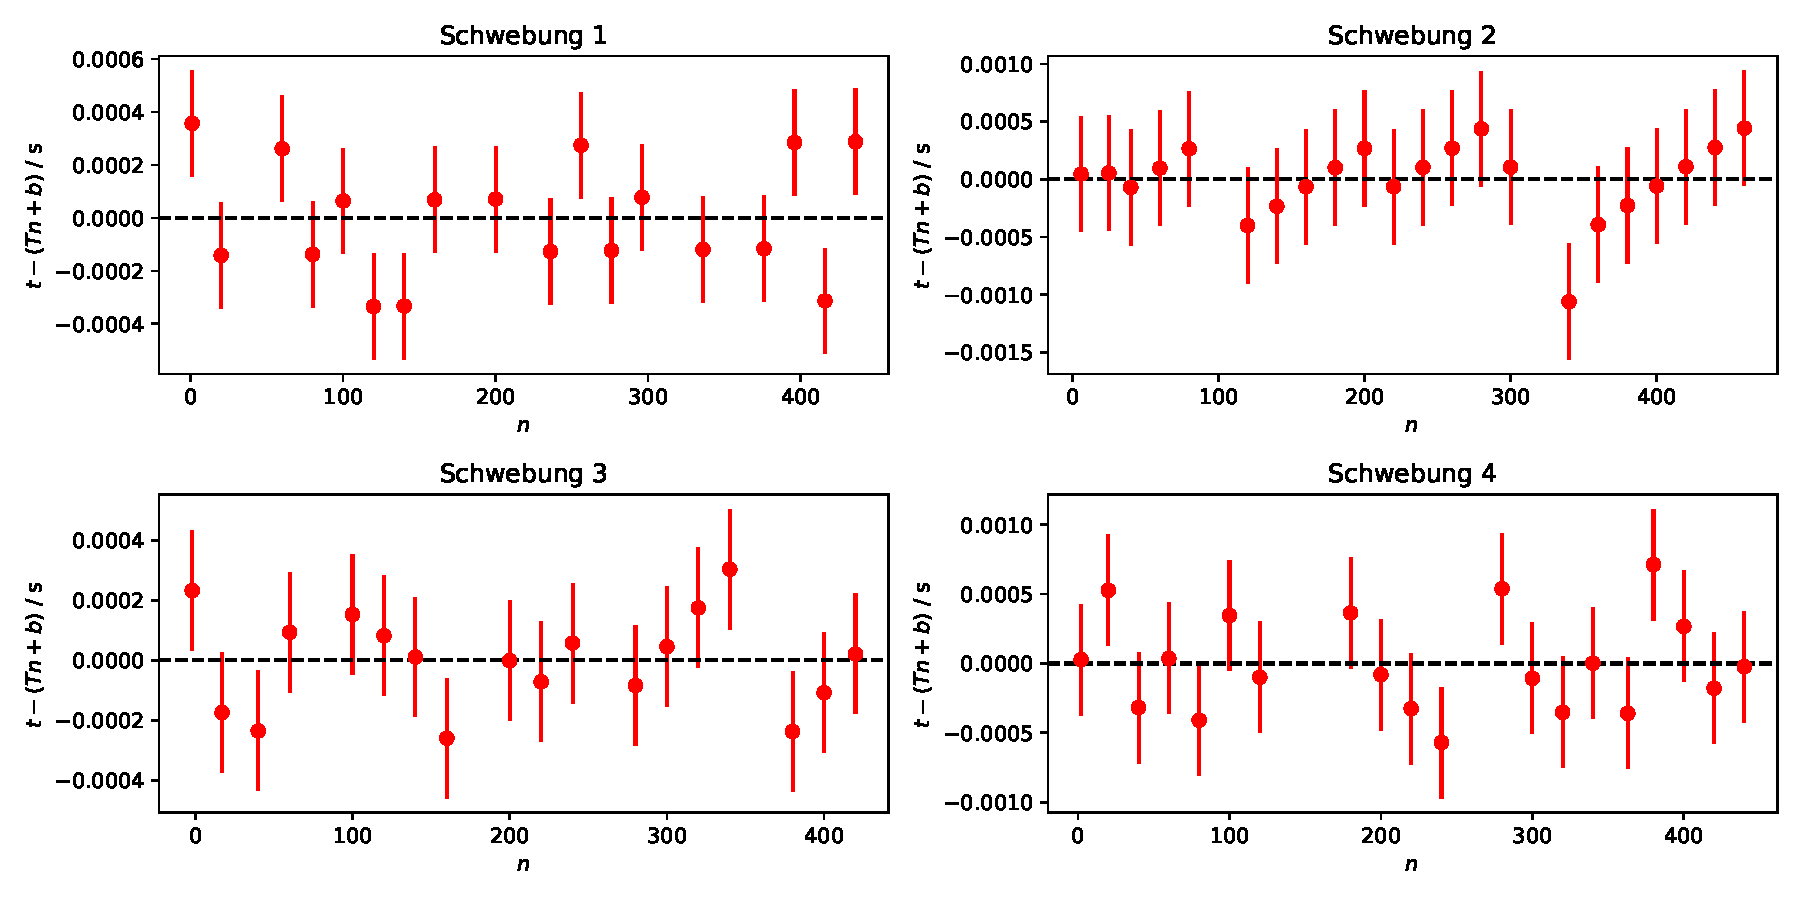
\includegraphics[width=\linewidth]{plots/residuenRes.pdf}
	\caption{Residuenplots der Regression für die resultierende Schwingung}
	\label{residuenRes}
\end{figure}

Bei Schwebung 2 könnte man eine Systematik vermuten. Es wurden jedoch die Abstände der Extrema bei den Sprüngen nochmals nachgeprüft. Nun werden die Zeitpunkte der Extrema der Schwebungsschwingung bestimmt. Die Zeiten sind in Tabelle \ref{tabTimeSch} aufgeführt. Für die Unsicherheiten der Zeitbestimmung wird für die Schwebungen 1 und 4 $\sigma_t = 0.005 \, \mathrm s$ und für die Schwebungen 2 und 3 $\sigma_t = 0.01 \, \mathrm s$ geschätzt.
\begin{table}[H]
\centering
\begin{tabular}{c|c|cccccccccc}
& $m$ & 1 & 2 & 3 & 4 & 5 & 6 & 7 & 8 & 9 & 10 \\
\hline
1 & \multirow{4}{*}{$t$ / s} & 0.155 & 0.465 & 0.780 & 1.085 & 1.410 & 1.720 & 2.035 & 2.345 & 2.655 & 2.975 \\
\cline{1-1}\cline{3-12}
2 & & 0.38 & 1.02 & 1.66 & 2.33 & 2.99 & & & & & \\
\cline{1-1}\cline{3-12}
3 & & 1.30 & 2.82 & & & & & & & & \\
\cline{1-1}\cline{3-12}
\multirow{3}{*}{4}
& & 0.075 & 0.240 & 0.420 & 0.595 & 0.760 & 0.930 & 1.100 & 1.270 & 1.445 & 1.620 \\
\cline{2-12}
& $m$ & 11 & 12 & 13 & 14 & 15 & 16 & 17 & 18 & & \\
\cline{2-12}
& $t$ / s & 1.795 & 1.965 & 2.135 & 2.305 & 2.470 & 2.640 & 2.810 & 2.975 & & 
\end{tabular}
\caption{Abgelesene Zeitpunkte für die Extrema der Schwebungsschwingung}
\label{tabTimeSch}
\end{table}
Wir erwarten wiederum einen linearen Zusammenhang $t(m) = \frac T2m + c$ mit der Periodendauer $T$ der Schwebungschwingung. Wir führen also eine lineare Regression durch mit den Resultaten in Tabelle \ref{tabRegressionSch}.

\begin{table}[H]
\centering
\begin{tabular}{c|c|c|c}
Schwebung & $T$ / ms & c & $\chi^2$ / $n_{df}$ \\
\hline
1 & $ 0.6266 \pm 0.0011$ & $ -0.161 \pm 0.003$ & 0.56 \\
2 & $ 1.3060 \pm 0.0063$ & $ -0.28 \pm 0.01$ & 1.43 \\
4 & $ 0.34211 \pm 0.00045$ & $ -0.094 \pm 0.003$ & 1.02
\end{tabular}
\caption{Ergebnisse der Regression für die Schwebungsschwingung}
\label{tabRegressionSch}
\end{table}
Da wir bei Schwebung 3 nur 2 Extrema vernünftig ablesen konnten, wird hier keine Regression gemacht, sondern die Periodendauer mittels $T = 2(t_2-t_1) = 3.04$ bestimmt. Die Unsicherheit beträgt dabei $\sigma_T = 2\sqrt{2} \sigma_t \approx 0.03$. Für die restlichen Schwebungen sind die Residuengraphen in Abbildung \ref{residuenSch}.

\begin{figure}[H]
	\centering
	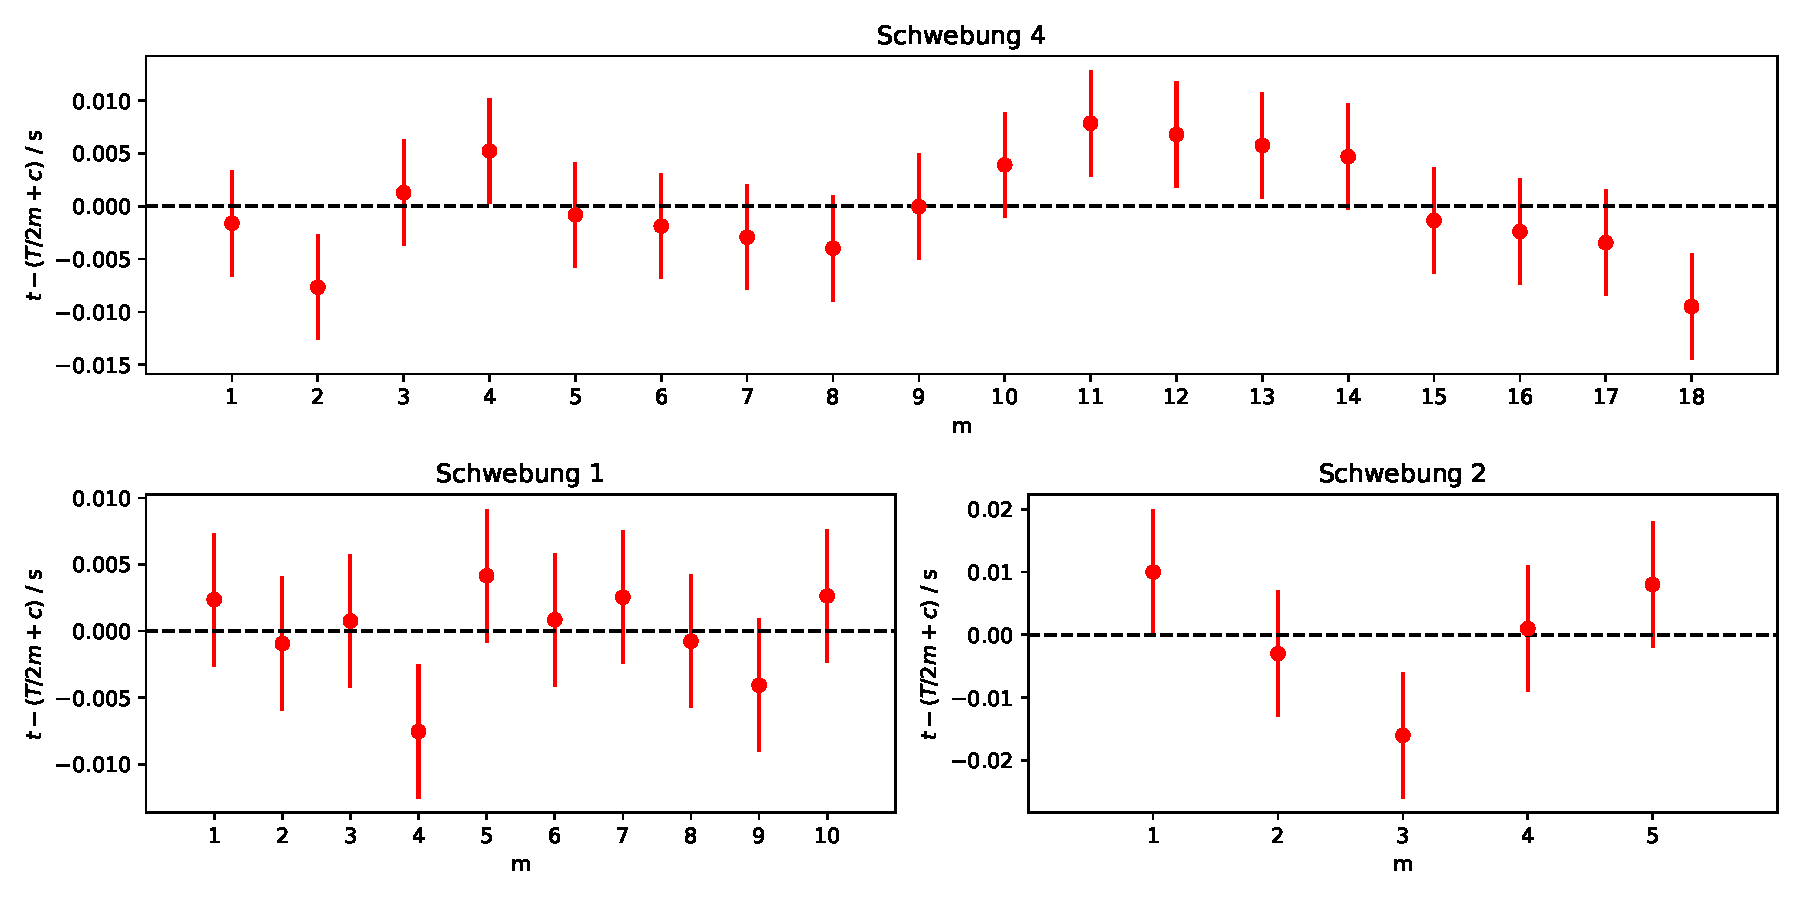
\includegraphics[width=\linewidth]{plots/residuenSch.pdf}
	\caption{Residuenplots der Regression für die Schwebungsschwingung}
	\label{residuenSch}
\end{figure}

Auf den ersten Blick sehen diese gut aus und es lässt sich keine Systematik erkennen.


Nun wollen wir uns dem Frequenzspektrum aus der FFT widmen. In Abbildung \ref{freqSpecSch} ist beispielhaft das Spektrum einer Schwebung abgebildet. Man sieht deutlich zwei Peaks bei etwa 145 Hz. Diese setzen sich zudem kleiner werdend bei den Vielfachen dieser Frequenz fort.
\begin{figure}[H]
	\centering
	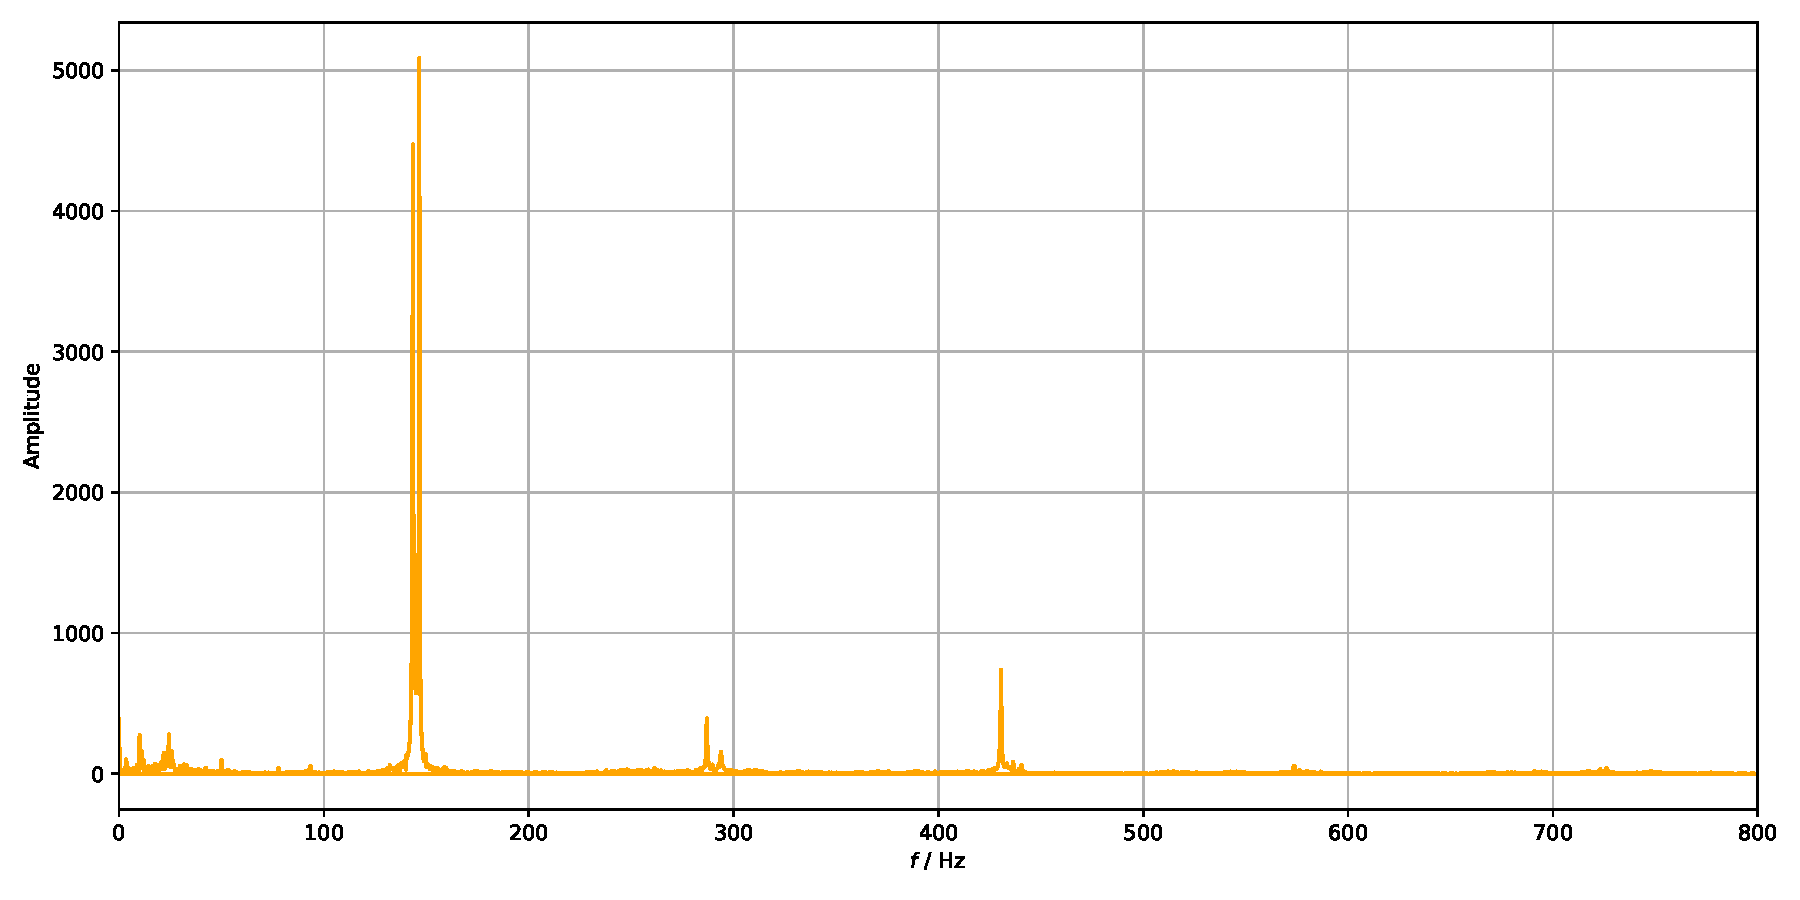
\includegraphics[width=\linewidth]{plots/schwebungsspektrum.pdf}
	\caption{Frequenzspektrum der ersten Messung (\mbox{``schwebung\_1.lab''})}
	\label{freqSpecSch}
\end{figure}

Wir benutzen nun die Peakfinder-Methode der Praktikumsbibliothek um die Frequenzen der Peaks zu bestimmen. Die Resultate sind in Abbildung \ref{fftPeakSch} für alle vier Schwebungen zu sehen.

\begin{figure}[H]
	\centering
	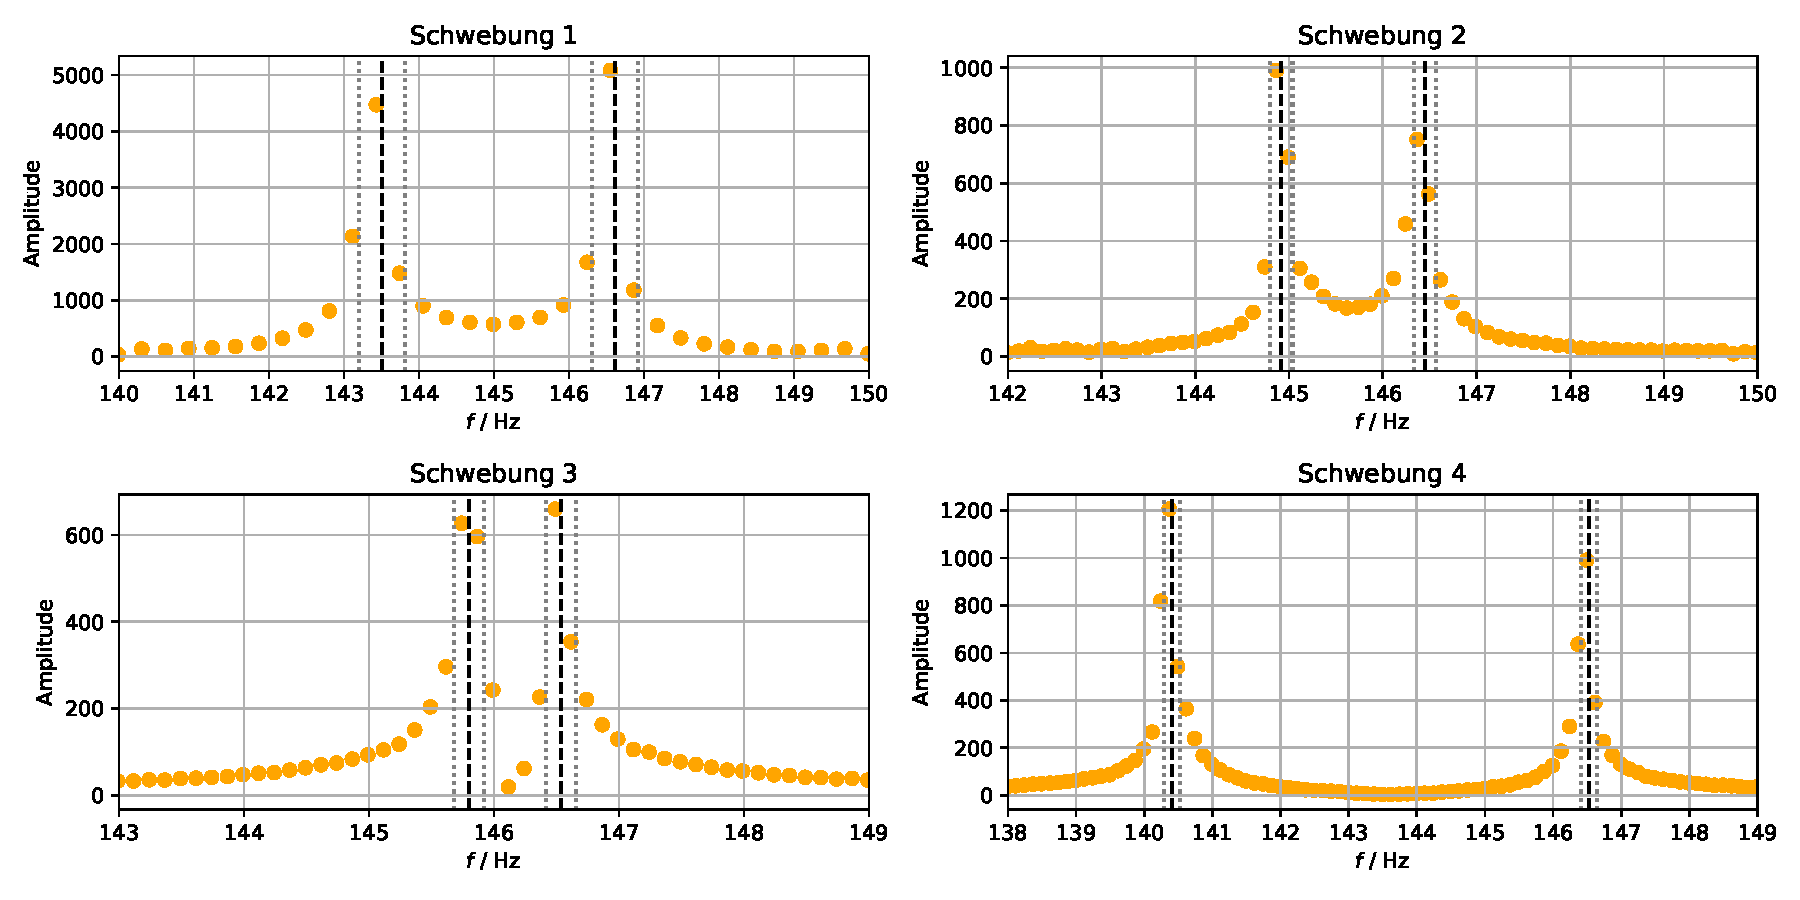
\includegraphics[width=\linewidth]{plots/FFT_freq.pdf}
	\caption{FFT der Schwebungen mit Peakanalyse}
	\label{fftPeakSch}
\end{figure}
Als Fehler wird dabei die Frequenzdifferenz zwischen zwei Punkten in der FFT genommen. Die Ergebnisse der Berechnungen sind in Tabelle \ref{tabFFTpeakSch} aufgelistet. Zudem ist dort auch angegeben auf welche Frequenzbereiche des Spektrums die Peakfinder-Methode angewendet wurde.

\begin{table}[H]
\centering
\begin{tabular}{c|c|c|c|c}
Schwebung & $f_1$ / Hz & Bereich für $f_1$ / Hz & $f_2$ / Hz & Bereich für $f_2$ / Hz \\
\hline
1 & $ 143.51 \pm 0.31$ & 142-145 & $ 146.61 \pm 0.31$ & 145-148 \\
2 & $ 144.92 \pm 0.12$ & 144-145.5 & $ 146.45 \pm 0.12$ & 145.5-147.5 \\
3 & $ 145.85 \pm 0.12$ & 144-146.2 & $ 146.47 \pm 0.12$ & 146.1-148 \\
4 & $ 140.40 \pm 0.12$ & 138-143.5 & $ 146.53 \pm 0.12$ & 143.5-149 
\end{tabular}
\caption{Ergebnisse der Peakanalyse der Frequenspektren}
\label{tabFFTpeakSch}
\end{table}
Mit diesen Werten lassen sich nun die Frequenz der resultierenden Schwingung und der Schwebungsschwingung berechnen, wenn man
$$f_S = \frac{f_2-f_1}2 \, , \hspace{1cm} f_R = \frac{f_2+f_1}2$$
benutzt. Berechnet man zusätzlich anhand der abgelesenen Periodendauern die Frequenzen mittels $f = \frac 1T$, so ergibt sich das Resultat in Tabelle \ref{tabFreqErg}.


\begin{table}[H]
\centering
\begin{tabular}{c|c|c|c|c}
& \multicolumn{2}{c|}{Abgelesen} & \multicolumn{2}{c}{FFT} \\
\hline
Schwebung & $f_S$ / Hz & $f_R$ / Hz & $f_S$ / Hz & $f_R$ / Hz \\
\hline
1 & $ 1.5959 \pm 0.0028$ & $ 144.9290 \pm 0.0074$ & $ 1.55 \pm 0.22$ & $ 145.06 \pm 0.22$ \\
2 & $ 0.7657 \pm 0.0037$ & $ 145.6978 \pm 0.0076$ & $ 0.77 \pm 0.08$ & $ 145.69 \pm 0.08$ \\
3 & $ 0.3289 \pm 0.0032$ & $ 146.164 \pm 0.016$ & $ 0.31 \pm 0.08$ & $ 146.16 \pm 0.08$ \\
4 & $ 2.9230 \pm 0.0038$ & $ 143.426 \pm 0.013$ & $ 3.07 \pm 0.08$ & $ 143.47 \pm 0.08$ 
\end{tabular}
\caption{Ergebnisse der Frequenzen von resultierender und Schwebungs-Schwingung}
\label{tabFreqErg}
\end{table}



\subsubsection{Fazit}

Wir haben nun auf zwei verschiedene Arten Werte für die Frequenzen der Schwebungschwingung und der resultierenden Scwhingung erhalten. Zum Vergleich der Werte berechnen wir die relativen Abweichungen.

\begin{table}[H]
\centering
\begin{tabular}{c|c|c|c|c|c|c|c|c}
& \multicolumn{4}{c|}{$f_S$} & \multicolumn{4}{c}{$f_R$} \\
\hline
Schwebung & 1 & 2 & 3 & 4 & 1 & 2 & 3 & 4 \\
\hline
$\frac{|f_1-f_2|}{\sqrt{\sigma_1^2+\sigma_2^2}}$ & 0.21 & 0.05 & 0.24 & 1.84 & 0.60 & 0.10 & 0.05 & 0.54 
\end{tabular}
\end{table}
Die Werte stimmen überwiegend gut überein. Bei Schwebung 4 liegen die Schwebungsfrequenzen $f_S$ weiter auseinander. Es könnte der Fehler bei der Auswertung mit der FFT unterschätzt worden. Ein Zusammenhang zur Verwendung von verschiedenen Messungen bei der Auswertung kann ausgeschlossen werden, da eine FFT der anderen Messung diegleichen Frequenzen liefert.  


\subsection{Aufnahme eines Frequenzspektrums}

\subsubsection{Versuchsdurchführung}


\subsubsection{Versuchsauswertung}

